\mode<presentation>{\gdef\figscale{1}}
\mode<article>{\gdef\figscale{0.5}}


\section{Decision Trees: Basic Idea}


\begin{frame}{Tree-Based Methods: Overview}
    \begin{itemize}
        \item Tree-based methods \textbf{stratify} (segment) the predictor space into a number of simple regions
        \item A new observation is predicted using the training observations in the region it belongs to: the \textbf{mean} response (regression) or the \textbf{most common class} (classification)
        \item The set of splitting rules can be summarised in a tree, hence the name \textbf{decision trees}
        \item A single tree is easy to interpret but is usually a weak predictor
% \item \textbf{Bagging}, \textbf{random forests}, \textbf{boosting} and \textbf{BART} combine many trees, trading interpretability for accuracy
        \item \textbf{Bagging}, \textbf{random forests} and \textbf{boosting} combine many trees, trading interpretability for accuracy
    \end{itemize}
\end{frame}


\section{Regression Trees}


\begin{frame}{Regression Trees: Example}
    \begin{center}
        \begin{tabular}{cc}
            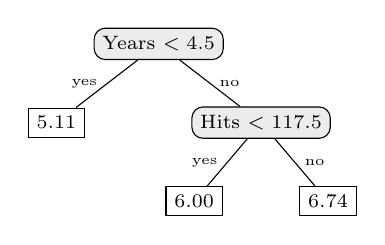
\begin{tikzpicture}[
                level distance=1.0cm,
                level 1/.style={sibling distance=2.6cm},
                level 2/.style={sibling distance=1.7cm},
                every node/.style={font=\scriptsize},
                split/.style={draw, rounded corners, fill=gray!15, inner sep=3pt},
                leaf/.style={draw, fill=white, inner sep=3pt}]
                \node[split] {Years $< 4.5$}
                    child {node[leaf] {$5.11$} edge from parent node[left, font=\tiny] {yes}}
                    child {node[split] {Hits $< 117.5$}
                        child {node[leaf] {$6.00$} edge from parent node[left, font=\tiny] {yes}}
                        child {node[leaf] {$6.74$} edge from parent node[right, font=\tiny] {no}}
                        edge from parent node[right, font=\tiny] {no}};
            \end{tikzpicture}
            &
            % figure produced by hitters.R
            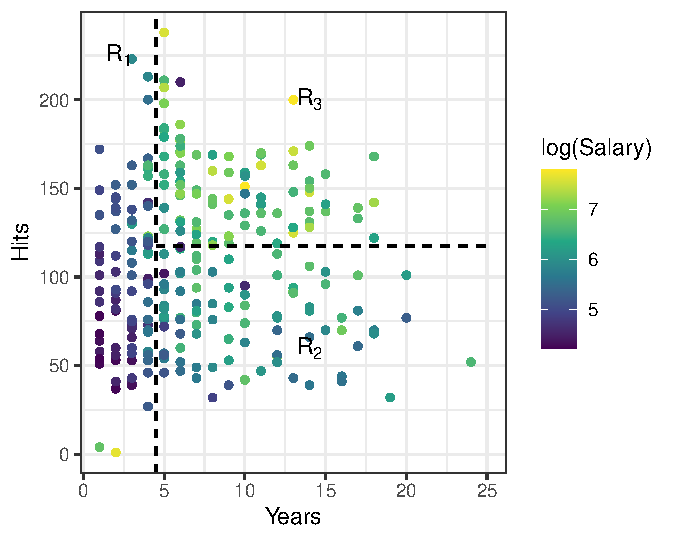
\includegraphics[width=0.4\linewidth]{figures/hitters_partition}
        \end{tabular}
    \end{center}
    \begin{itemize}
        \item Response $\log(\text{Salary})$; predictors \texttt{Years} in the major leagues and \texttt{Hits} in the previous year; each leaf shows the mean response in its region
        \item Years is the most important factor; Hits matters only for experienced players
    \end{itemize}
\end{frame}


\begin{frame}{Regression Trees: Prediction and Objective}
    \begin{itemize}
        \item Divide the predictor space into $J$ distinct, non-overlapping regions $R_1, \dots, R_J$
        \item Every observation falling in $R_m$ receives the same prediction, the mean response of the training observations in $R_m$
    \end{itemize}
    \[
        \hat{y}_{R_m} = \frac{1}{|R_m|} \sum_{i:\, \mathbf{x}^{(i)} \in R_m} y^{(i)}, \qquad
        \hat{f}(\mathbf{x}) = \sum_{m=1}^{J} \hat{y}_{R_m}\, \mathrm{I}(\mathbf{x} \in R_m)
    \]
    \begin{itemize}
        \item Regions are chosen as high-dimensional \textbf{boxes} (rectangles) for simplicity and interpretability
        \item Goal: find boxes that minimise the residual sum of squares
    \end{itemize}
    \[
        \mathrm{RSS} = \sum_{m=1}^{J} \sum_{i:\, \mathbf{x}^{(i)} \in R_m} \left( y^{(i)} - \hat{y}_{R_m} \right)^2
    \]
\end{frame}


\begin{frame}{Recursive Binary Splitting}
    \begin{itemize}
        \item Considering every possible partition into $J$ boxes is infeasible; use a \textbf{top-down, greedy} approach
        \item For predictor $j$ and cutpoint $s$, define the pair of half-planes
    \end{itemize}
    \[
        R_1(j, s) = \{ \mathbf{x} \mid x_j < s \} \quad \text{and} \quad R_2(j, s) = \{ \mathbf{x} \mid x_j \ge s \}
    \]
    \begin{itemize}
        \item Choose $j$ and $s$ that minimise
    \end{itemize}
    \[
        \sum_{i:\, \mathbf{x}^{(i)} \in R_1(j,s)} \left( y^{(i)} - \hat{y}_{R_1} \right)^2 + \sum_{i:\, \mathbf{x}^{(i)} \in R_2(j,s)} \left( y^{(i)} - \hat{y}_{R_2} \right)^2
    \]
\end{frame}


\begin{frame}{Recursive Binary Splitting: Greedy Search and Stopping}
    \begin{itemize}
        \item \textbf{Greedy}: the best split at the current step is chosen, even if a mediocre split now would enable a better one later
        \item After the first split, repeat the search inside each of the two resulting regions: choose the region, predictor $j$ and cutpoint $s$ that reduce the RSS the most
        \item Continue until a stopping criterion is met, e.g. no region has more than five observations
        \item The final regions $R_1, \dots, R_J$ are the leaves of the tree, and a test observation is predicted by the mean response of the region it falls in
    \end{itemize}
\end{frame}


% Panel showing the partition of a two-dimensional predictor space after #1 splits (0 to 4)
\newcommand{\partpanel}[1]{%
    \begin{tikzpicture}[scale=0.5, every node/.style={font=\tiny}]
        \draw (0,0) rectangle (4,4);
        \node[below] at (2,0) {$X_1$};
        \node[left] at (0,2) {$X_2$};
        \ifnum#1>0 \draw[thick] (1.5,0) -- (1.5,4); \node[above] at (1.5,4) {$t_1$}; \fi
        \ifnum#1>1 \draw[thick] (1.5,1.2) -- (4,1.2); \node[right] at (4,1.2) {$t_2$}; \fi
        \ifnum#1>2 \draw[thick] (2.8,1.2) -- (2.8,4); \node[above] at (2.8,4) {$t_3$}; \fi
        \ifnum#1>3 \draw[thick] (2.8,2.8) -- (4,2.8); \node[right] at (4,2.8) {$t_4$}; \fi
        \ifnum#1>3
            \node at (0.75,2) {$R_1$};
            \node at (2.75,0.6) {$R_2$};
            \node at (2.15,2.6) {$R_3$};
            \node at (3.4,2.0) {$R_4$};
            \node at (3.4,3.4) {$R_5$};
        \fi
    \end{tikzpicture}}


\begin{frame}{Building the Partition Step by Step}
    \begin{center}
        \begin{tabular}{cccc}
            \partpanel{1} & \partpanel{2} & \partpanel{3} & \partpanel{4} \\
            \footnotesize 1st split & \footnotesize 2nd split & \footnotesize 3rd split & \footnotesize 4th split
        \end{tabular}
    \end{center}
    \begin{itemize}
        \item The first split divides the whole space in two by a line perpendicular to one predictor axis
        \item Each later split divides \emph{one} existing region, never the whole space
        \item Every split is a straight line parallel to a coordinate axis, so the final regions are boxes
        \item Each split is chosen to reduce RSS the most, given the splits made so far
    \end{itemize}
\end{frame}


\begin{frame}{Partition, Tree and Invalid Partitions}
    \begin{center}
        \begin{tabular}{ccc}
            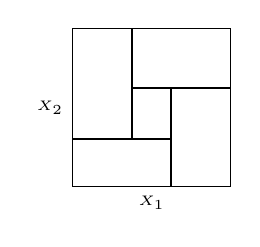
\begin{tikzpicture}[scale=0.5, every node/.style={font=\tiny}]
                \draw (0,0) rectangle (4,4);
                \draw[thick] (0,1.2) -- (2.5,1.2);
                \draw[thick] (2.5,0) -- (2.5,2.5);
                \draw[thick] (1.5,2.5) -- (4,2.5);
                \draw[thick] (1.5,1.2) -- (1.5,4);
                \draw[thick] (1.5,1.2) rectangle (2.5,2.5);
                \node[below] at (2,0) {$X_1$};
                \node[left] at (0,2) {$X_2$};
            \end{tikzpicture}
            &
            \partpanel{4}
            &
            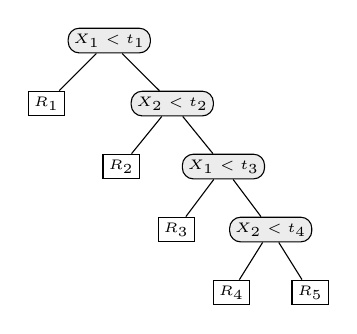
\begin{tikzpicture}[
                level distance=0.8cm,
                level 1/.style={sibling distance=1.6cm},
                level 2/.style={sibling distance=1.3cm},
                level 3/.style={sibling distance=1.2cm},
                level 4/.style={sibling distance=1.0cm},
                every node/.style={font=\tiny},
                split/.style={draw, rounded corners, fill=gray!15, inner sep=2pt},
                leaf/.style={draw, fill=white, inner sep=2pt}]
                \node[split] {$X_1 < t_1$}
                    child {node[leaf] {$R_1$}}
                    child {node[split] {$X_2 < t_2$}
                        child {node[leaf] {$R_2$}}
                        child {node[split] {$X_1 < t_3$}
                            child {node[leaf] {$R_3$}}
                            child {node[split] {$X_2 < t_4$}
                                child {node[leaf] {$R_4$}}
                                child {node[leaf] {$R_5$}}}}};
            \end{tikzpicture}
            \\[2pt]
            \shortstack{\footnotesize Cannot result from\\ \footnotesize recursive binary splitting}
            & \shortstack{\footnotesize Can result from\\ \footnotesize recursive binary splitting}
            & \shortstack{\footnotesize The tree for the\\ \footnotesize middle partition}
        \end{tabular}
    \end{center}
    \begin{itemize}
        \item The left partition has no first split that cuts the whole space cleanly into two unions of its regions
        \item The tree is read top to bottom: left branch if the condition is true, right branch otherwise
    \end{itemize}
\end{frame}


\begin{frame}{Overfitting and Tree Pruning}
    \begin{itemize}
        \item The resulting large tree fits the training data very well but overfits: high variance, poor test performance
        \item A smaller tree with fewer splits has lower variance and better interpretability at the cost of a little bias
        \item Stopping when the RSS decrease from a split is small is short-sighted, since a poor split may be followed by a very good one
        \item Better: grow a large tree $T_0$, then \textbf{prune} it back to obtain a subtree
    \end{itemize}
\end{frame}


\begin{frame}{Cost Complexity Pruning}
    \begin{itemize}
        \item For each tuning parameter $\alpha \ge 0$, there is a subtree $T \subseteq T_0$ that minimises
    \end{itemize}
    \[
        \sum_{m=1}^{|T|} \sum_{i:\, \mathbf{x}^{(i)} \in R_m} \left( y^{(i)} - \hat{y}_{R_m} \right)^2 + \alpha\, |T|
    \]
    \begin{itemize}
        \item $|T|$ is the number of terminal nodes (leaves) of $T$, and $R_m$ is the region of the $m$-th leaf
        \item $\alpha$ controls the trade-off between fit to the training data and tree complexity
        \item $\alpha = 0$ gives $T_0$; as $\alpha$ increases, branches are pruned in a nested and predictable way, giving the whole sequence of subtrees
        \item Similar in spirit to the lasso, which penalises the size of the coefficients
    \end{itemize}
\end{frame}


\begin{frame}{Building a Regression Tree}
    \begin{enumerate}
        \item Use recursive binary splitting to grow a large tree on the training data, stopping when each leaf has fewer than some minimum number of observations
        \item Apply cost complexity pruning to obtain the sequence of best subtrees as a function of $\alpha$
        \item Use $K$-fold cross-validation to choose $\alpha$: for each fold, repeat steps 1 and 2 on the other $K-1$ folds and evaluate the MSE on the held-out fold as a function of $\alpha$; average over folds and pick the $\alpha$ with the smallest CV error
        \item Return the subtree from step 2 that corresponds to the chosen $\alpha$
    \end{enumerate}
\end{frame}


\begin{frame}{Regression Tree: Choosing the Tree Size}
    \begin{columns}[T]
        \begin{column}{0.55\textwidth}
            % figure produced by hitters.R
            \centerline{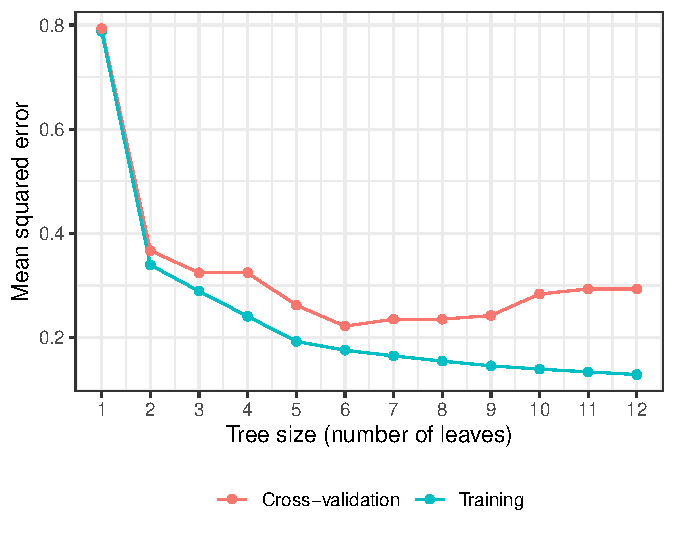
\includegraphics[width=\figscale\linewidth]{figures/hitters_cv}}
        \end{column}
        \begin{column}{0.45\textwidth}
            \begin{itemize}
                \item Hitters data with nine predictors, trees of increasing size
                \item Training error decreases monotonically with the number of leaves
                \item CV error is U-shaped; it picks a small tree
                \item The selected tree is simple and interpretable
            \end{itemize}
        \end{column}
    \end{columns}
\end{frame}


\begin{frame}{Hyperparameters and Tuning: Background}
    \begin{itemize}
        \item \textbf{Parameters} are learned from the training data, e.g. the splits and leaf means of a tree
        \item \textbf{Hyperparameters} are set \emph{before} fitting and control model flexibility, e.g. the pruning parameter $\alpha$, the number of trees $B$, the number of predictors $m$ per split, the shrinkage $\lambda$ and the depth $d$
        \item Training error always favours the most flexible setting (e.g. $\alpha = 0$ gives the largest tree), so hyperparameters must be chosen using an estimate of the \textbf{test} error
        \item The test set must not be used for this, otherwise it no longer gives an honest estimate of the final model's performance
    \end{itemize}
\end{frame}


\begin{frame}{Hyperparameter Tuning: Procedure}
    \begin{enumerate}
        \item Choose a grid $\Gamma$ of candidate values; with several hyperparameters, use all combinations (grid search) or a random sample of them (random search)
        \item For each candidate $\symbf{\gamma} \in \Gamma$, estimate the test error using a validation set or $K$-fold cross-validation
        \item Choose the candidate with the smallest estimated error
        \item Refit the model on the whole training set with the chosen $\hat{\symbf{\gamma}}$, and evaluate it once on the test set
    \end{enumerate}
    \[
        \hat{\symbf{\gamma}} = \operatorname*{arg\,min}_{\symbf{\gamma} \in \Gamma}\, \mathrm{CV}_{(K)}(\symbf{\gamma}), \qquad
        \mathrm{CV}_{(K)}(\symbf{\gamma}) = \frac{1}{K} \sum_{k=1}^{K} \mathrm{Err}_k(\symbf{\gamma})
    \]
    \begin{itemize}
        \item $\mathrm{Err}_k(\symbf{\gamma})$ is the error on fold $k$ of a model fit with $\symbf{\gamma}$ on the other $K-1$ folds
        \item The cost grows with the number of candidates times $K$ model fits
    \end{itemize}
\end{frame}


\section{Classification Trees}


\begin{frame}{Classification Trees}
    \begin{itemize}
        \item Same as a regression tree, but the response is qualitative with classes $k = 1, \dots, K$
        \item The prediction for an observation is the most commonly occurring class among the training observations in its region
        \item Let $\hat{p}_{mk}$ be the proportion of training observations in region $R_m$ that belong to class $k$
    \end{itemize}
    \[
        \hat{p}_{mk} = \frac{1}{|R_m|} \sum_{i:\, \mathbf{x}^{(i)} \in R_m} \mathrm{I}\left( y^{(i)} = k \right), \qquad
        \hat{y}_{R_m} = \operatorname*{arg\,max}_{k}\, \hat{p}_{mk}
    \]
    \begin{itemize}
        \item RSS cannot be used as the splitting criterion, so we need a measure of how \emph{mixed} the classes are in a node
    \end{itemize}
\end{frame}


\begin{frame}{Node Impurity Measures}
    \begin{itemize}
        \item \textbf{Classification error rate}: fraction of training observations in the region not in the majority class
    \end{itemize}
    \[
        E_m = 1 - \max_{k}\, \hat{p}_{mk}
    \]
    \begin{itemize}
        \item \textbf{Gini index}: total variance across the $K$ classes
    \end{itemize}
    \[
        G_m = \sum_{k=1}^{K} \hat{p}_{mk} \left( 1 - \hat{p}_{mk} \right)
    \]
    \begin{itemize}
        \item \textbf{Entropy}
    \end{itemize}
    \[
        D_m = - \sum_{k=1}^{K} \hat{p}_{mk} \log \hat{p}_{mk}
    \]
\end{frame}


\begin{frame}{Gini and Entropy as Measures of Node Purity}
    \begin{columns}[T]
        \begin{column}{0.5\textwidth}
            % figure produced by simulated.R
            \centerline{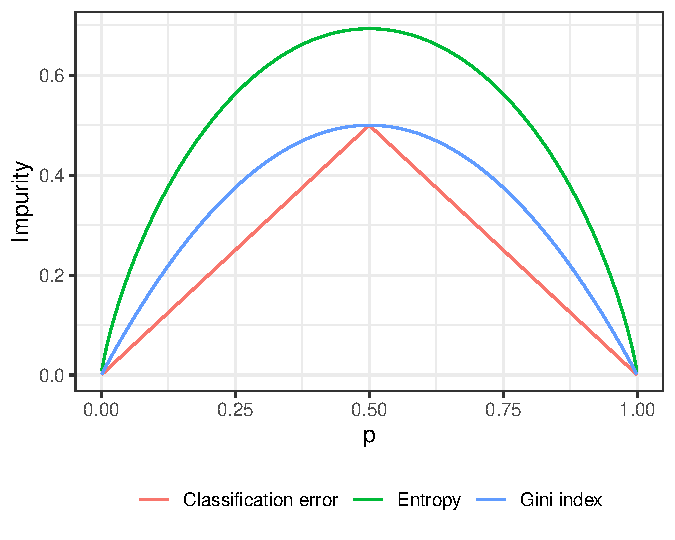
\includegraphics[width=\figscale\linewidth]{figures/impurity}}
        \end{column}
        \begin{column}{0.5\textwidth}
            \begin{itemize}
                \item Two classes, with $p$ the proportion in class 1
                \item $G_m$ and $D_m$ are small when all $\hat{p}_{mk}$ are close to 0 or 1, so a small value indicates a \textbf{pure} node
                \item Gini and entropy are numerically very similar
                \item Both are differentiable and more sensitive to node purity than the error rate, which is piecewise linear in $p$
            \end{itemize}
        \end{column}
    \end{columns}
\end{frame}


\begin{frame}{Choosing a Split: Worked Example}
    \begin{itemize}
        \item Parent node with 400 observations in each of two classes; compare two candidate splits, each with (class 1, class 2) counts in the left and right child
        \item A split is scored by the size-weighted impurity of its children
    \end{itemize}
    \[
        \frac{n_L}{n_L + n_R}\, Q_L + \frac{n_R}{n_L + n_R}\, Q_R, \qquad Q \in \{E, G, D\}
    \]
    \begin{center}
        \small
        \begin{tabular}{lcccc}
            \hline
            & Left & Right & Gini $G$ & Entropy $D$ \\
            \hline
            Split A & $(300, 100)$ & $(100, 300)$ & $0.375$ & $0.562$ \\
            Split B & $(200, 400)$ & $(200, 0)$ & $0.333$ & $0.477$ \\
            \hline
        \end{tabular}
    \end{center}
    \begin{itemize}
        \item Both splits have the same error rate, $E = 0.25$, but Gini and entropy prefer split B because it creates a pure node
    \end{itemize}
\end{frame}


\begin{frame}{Growing and Pruning Classification Trees}
    \begin{itemize}
        \item When \textbf{growing} the tree, the Gini index or entropy is preferred, because they are more sensitive to node purity
        \item When \textbf{pruning}, any of the three can be used, but the classification error rate is preferable if the goal is prediction accuracy
        \item A split can leave both children with the same predicted class and still be worthwhile: it increases purity, hence our confidence in the prediction
        \item The pruning parameter $\alpha$ is chosen by cross-validation, exactly as for regression trees
    \end{itemize}
\end{frame}


\begin{frame}{Classification Tree: Heart Data}
    \begin{columns}[T]
        \begin{column}{0.55\textwidth}
            % figure produced by heart.R
            \centerline{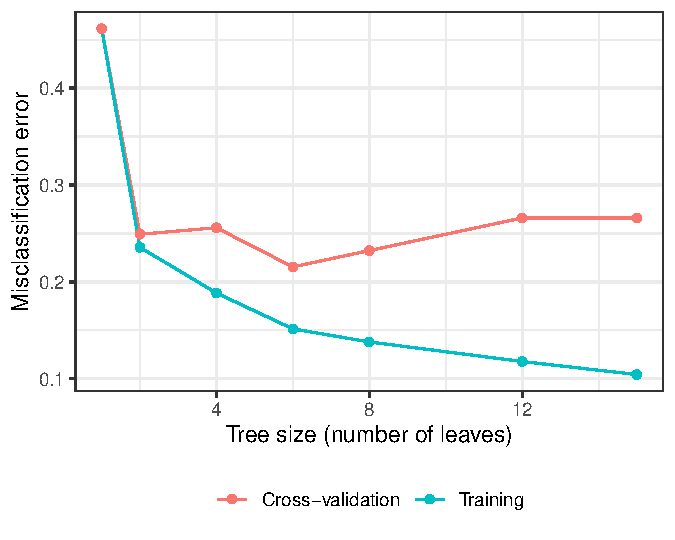
\includegraphics[width=\figscale\linewidth]{figures/heart_cv}}
        \end{column}
        \begin{column}{0.45\textwidth}
            \begin{itemize}
                \item Binary outcome: heart disease (\texttt{AHD}) \texttt{Yes}/\texttt{No}, with 13 predictors
                \item Training error keeps falling as the tree grows
                \item CV error flattens or rises beyond a small tree
                \item The pruned tree has comparable accuracy to the full tree and is much easier to read
            \end{itemize}
        \end{column}
    \end{columns}
\end{frame}


\begin{frame}{Qualitative Predictors in Trees}
    \begin{itemize}
        \item A split on a qualitative predictor assigns some of its levels to one branch and the rest to the other, e.g. \texttt{ChestPain} $\in \{\text{typical}, \text{nonanginal}\}$
        \item No dummy variables are needed
        \item A predictor with $L$ unordered levels admits $2^{L-1} - 1$ distinct binary splits
        \item Splits on quantitative predictors only depend on the ordering of the values, so trees are unaffected by monotone transformations and need no scaling
    \end{itemize}
\end{frame}


\begin{frame}{Trees Versus Linear Models}
    \begin{columns}[T]
        \begin{column}{0.5\textwidth}
            % \begin{itemize}
            %     \item Linear regression assumes
            % \end{itemize}
            % \[
            %     f(\mathbf{x}) = \beta_0 + \sum_{j=1}^{p} x_j \beta_j
            % \]
            % \begin{itemize}
            %     \item Regression trees assume
            % \end{itemize}
            % \[
            %     f(\mathbf{x}) = \sum_{m=1}^{J} c_m\, \mathrm{I}(\mathbf{x} \in R_m)
            % \]
            \begin{itemize}
                \item The better model depends on the shape of the true boundary
                \item Approximately linear boundary: linear model wins; highly non-linear, axis-aligned structure: tree wins
            \end{itemize}
        \end{column}
        \begin{column}{0.5\textwidth}
            % figure produced by simulated.R
            \centerline{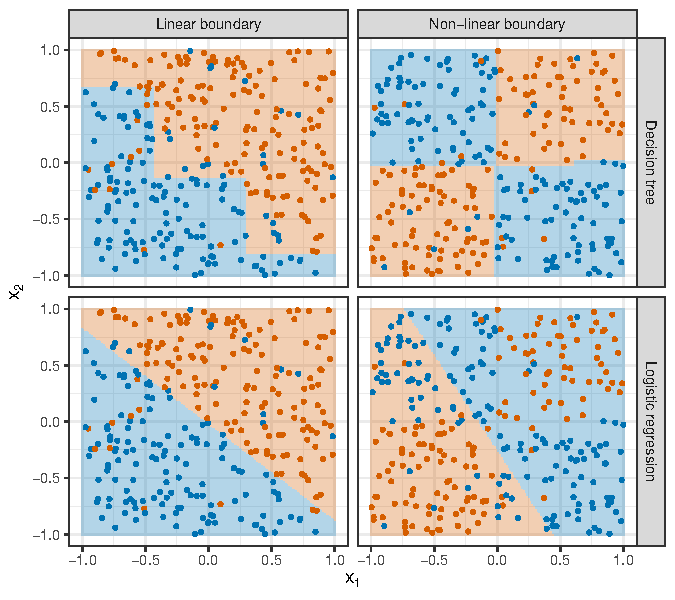
\includegraphics[width=\figscale\linewidth]{figures/tree_vs_linear}}
        \end{column}
    \end{columns}
    % \begin{itemize}
    %     \item Approximately linear boundary: linear model wins; highly non-linear, axis-aligned structure: tree wins
    % \end{itemize}
\end{frame}


\begin{frame}{Advantages and Disadvantages of Trees}
    \begin{columns}[T]
        \begin{column}{0.5\textwidth}
            \textbf{Advantages}
            \begin{itemize}
                \item Very easy to explain
                \item Closely mirror human decision-making
                \item Displayed graphically, easy to interpret
                \item Handle qualitative predictors without dummy variables
            \end{itemize}
        \end{column}
        \begin{column}{0.5\textwidth}
            \textbf{Disadvantages}
            \begin{itemize}
                \item Predictive accuracy is generally lower than other regression and classification methods
                \item Non-robust: a small change in the data can cause a large change in the final tree, i.e.\ high variance
            \end{itemize}
        \end{column}
    \end{columns}
    \vspace{1em}
    Aggregating many trees can substantially improve predictive performance.
\end{frame}


% \section{Ensemble Methods: Bagging, Random Forests, Boosting and BART}
\section{Ensemble Methods: Bagging, Random Forests and Boosting}


\begin{frame}{The Bootstrap: Background}
    \begin{itemize}
        \item We have only one dataset, but want to know how an estimate (e.g.\ a mean or a tree's prediction) would change on other datasets
        \item The \textbf{bootstrap} creates new datasets by sampling $n$ observations \textbf{with replacement} from the original $n$ observations
        \item Some observations appear several times in a bootstrap dataset, others not at all
        \item Repeating this $B$ times gives $B$ bootstrap datasets, and the estimate computed on each shows how much it varies
    \end{itemize}
\end{frame}


\begin{frame}{The Bootstrap: Illustration}
    \begin{center}
        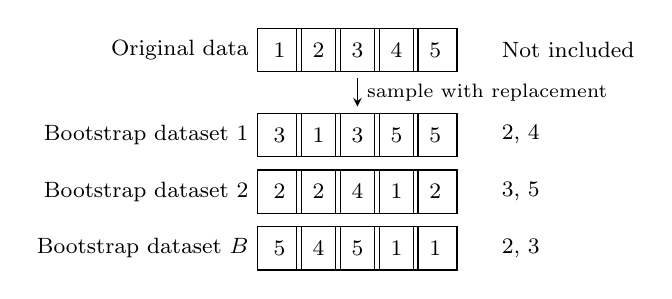
\begin{tikzpicture}[scale=0.9,
            box/.style={draw, minimum size=0.55cm, inner sep=0pt, font=\footnotesize},
            lab/.style={font=\footnotesize, anchor=east},
            >=stealth]
            \node[lab] at (-0.3,0) {Original data};
            \foreach \x/\v in {0/1, 0.55/2, 1.1/3, 1.65/4, 2.2/5} \node[box] at (\x,0) {\v};
            \node[font=\footnotesize, anchor=west] at (3.0,0) {Not included};
            \node[lab] at (-0.3,-1.2) {Bootstrap dataset 1};
            \foreach \x/\v in {0/3, 0.55/1, 1.1/3, 1.65/5, 2.2/5} \node[box] at (\x,-1.2) {\v};
            \node[font=\footnotesize, anchor=west] at (3.0,-1.2) {2, 4};
            \node[lab] at (-0.3,-2.0) {Bootstrap dataset 2};
            \foreach \x/\v in {0/2, 0.55/2, 1.1/4, 1.65/1, 2.2/2} \node[box] at (\x,-2.0) {\v};
            \node[font=\footnotesize, anchor=west] at (3.0,-2.0) {3, 5};
            \node[lab] at (-0.3,-2.8) {Bootstrap dataset $B$};
            \foreach \x/\v in {0/5, 0.55/4, 1.1/5, 1.65/1, 2.2/1} \node[box] at (\x,-2.8) {\v};
            \node[font=\footnotesize, anchor=west] at (3.0,-2.8) {2, 3};
            \draw[->] (1.1,-0.4) -- (1.1,-0.8) node[midway, right, font=\scriptsize] {sample with replacement};
        \end{tikzpicture}
    \end{center}
    \begin{itemize}
        \item Numbers are observation indices: each bootstrap dataset repeats some observations and omits others, e.g.\ dataset 1 contains observations 3 and 5 twice and omits 2 and 4
        \item Compute the estimate on each bootstrap dataset; the spread of these $B$ estimates measures its uncertainty
    \end{itemize}
\end{frame}


\begin{frame}{Reducing Variance by Averaging}
    \begin{itemize}
        \item Given independent random variables $Z_1, \dots, Z_n$, each with variance $\sigma^2$, the mean has a smaller variance
    \end{itemize}
    \[
        \operatorname{Var}(\bar{Z}) = \frac{\sigma^2}{n}
    \]
    \begin{itemize}
        \item Analogy: fit a separate tree on many training sets, then average the predictions to reduce variance
        \item We do not have many training sets, so we create pseudo-training sets using the \textbf{bootstrap}: sample $n$ observations with replacement from the training data
    \end{itemize}
\end{frame}


\begin{frame}{Bagging}
    \begin{itemize}
        \item \textbf{B}ootstrap \textbf{agg}regat\textbf{ing}: draw $B$ bootstrap samples, fit a tree $\hat{f}^{(b)}$ to the $b$-th sample, and average
    \end{itemize}
    \[
        \hat{f}_{\mathrm{bag}}(\mathbf{x}) = \frac{1}{B} \sum_{b=1}^{B} \hat{f}^{(b)}(\mathbf{x})
    \]
    \begin{itemize}
        \item Trees are grown deep and \textbf{not pruned}: each has high variance but low bias, and averaging reduces the variance
        \item For classification, take a \textbf{majority vote} over the $B$ predicted classes
        \item Using a large $B$ does not lead to overfitting; choose $B$ large enough that the error has settled
    \end{itemize}
\end{frame}


\begin{frame}{Out-of-Bag Error Estimation}
    \begin{itemize}
        \item The probability that observation $i$ appears in a given bootstrap sample is
    \end{itemize}
    \[
        1 - \left( 1 - \frac{1}{n} \right)^{n} \xrightarrow{n \to \infty} 1 - e^{-1} \approx 0.632
    \]
    \begin{itemize}
        \item So each tree uses about two-thirds of the observations; the remaining third are \textbf{out-of-bag} (OOB)
        \item Predict observation $i$ using only the trees for which it was OOB (about $B/3$ trees), by averaging or majority vote
        \item The OOB MSE or classification error is a valid estimate of test error, since each prediction uses a model that never saw the observation
        \item For large $B$ it is essentially equivalent to leave-one-out cross-validation, with no refitting
    \end{itemize}
\end{frame}


\begin{frame}{Variable Importance}
    \begin{columns}[T]
        \begin{column}{0.5\textwidth}
            \begin{itemize}
                \item A bagged ensemble is no longer a single readable tree
                \item \textbf{Variable importance}: the total decrease in RSS (regression) or Gini index (classification) due to splits on a predictor, averaged over all $B$ trees
                \item A large value indicates an important predictor
            \end{itemize}
        \end{column}
        \begin{column}{0.5\textwidth}
            % figure produced by heart.R
            \centerline{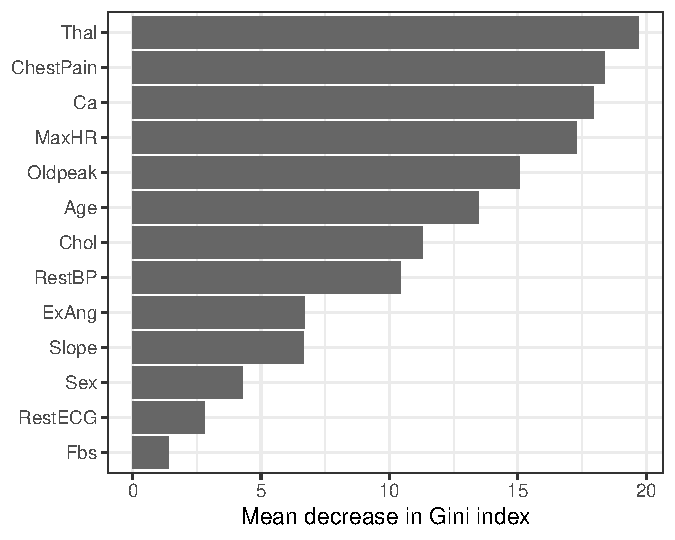
\includegraphics[width=\figscale\linewidth]{figures/heart_importance}}
        \end{column}
    \end{columns}
\end{frame}


\begin{frame}{Random Forests}
    \begin{itemize}
        \item If there is one very strong predictor, most bagged trees split on it first, so their predictions are highly correlated
        \item For $B$ identically distributed variables with variance $\sigma^2$ and pairwise correlation $\rho$
    \end{itemize}
    \[
        \operatorname{Var}\left( \frac{1}{B} \sum_{b=1}^{B} Z_b \right) = \rho\, \sigma^2 + \frac{1 - \rho}{B}\, \sigma^2
    \]
    \begin{itemize}
        \item As $B \to \infty$ the variance does not go below $\rho \sigma^2$, so correlated trees limit the gain from averaging
        \item \textbf{Random forests} \textbf{decorrelate} the trees: at each split only a random subset of $m$ of the $p$ predictors is considered
        \item Typical choice: $m \approx \sqrt{p}$ for classification and $m \approx p/3$ for regression; $m = p$ is bagging
    \end{itemize}
\end{frame}


\begin{frame}{Bagging Versus Random Forests: Heart Data}
    \begin{columns}[T]
        \begin{column}{0.55\textwidth}
            % figure produced by heart.R
            \centerline{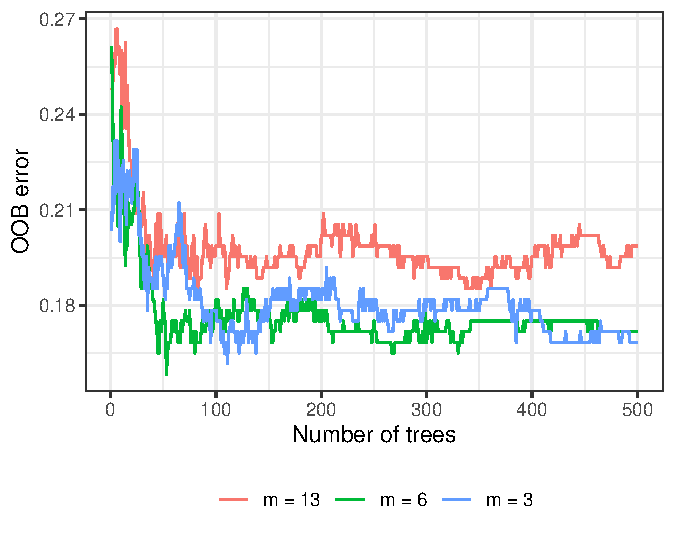
\includegraphics[width=\figscale\linewidth]{figures/heart_rf_oob}}
        \end{column}
        \begin{column}{0.45\textwidth}
            \begin{itemize}
                \item OOB error against the number of trees for $m = p$ (bagging), $p/2$ and $\sqrt{p}$
                \item Error stabilises after a modest number of trees
                \item Smaller $m$ often helps, especially with many correlated predictors
            \end{itemize}
        \end{column}
    \end{columns}
\end{frame}


\begin{frame}{Random Forests: Tuning Parameters}
    \begin{columns}[T]
        \begin{column}{0.5\textwidth}
            \begin{itemize}
                \item \textbf{Number of trees} $B$: as in bagging, a larger $B$ does not overfit; take it large enough that the error has settled
                \item \textbf{Predictors per split} $m$: the main tuning parameter; start from $\sqrt{p}$ (classification) or $p/3$ (regression) and try other values between $1$ and $p$
                \item \textbf{Minimum node size}: trees are grown deep and not pruned, so this is usually left small
                % \item Choose $m$ by the smallest OOB error, which needs no extra cross-validation
            \end{itemize}
        \end{column}
        \begin{column}{0.5\textwidth}
            % figure produced by heart.R
            \centerline{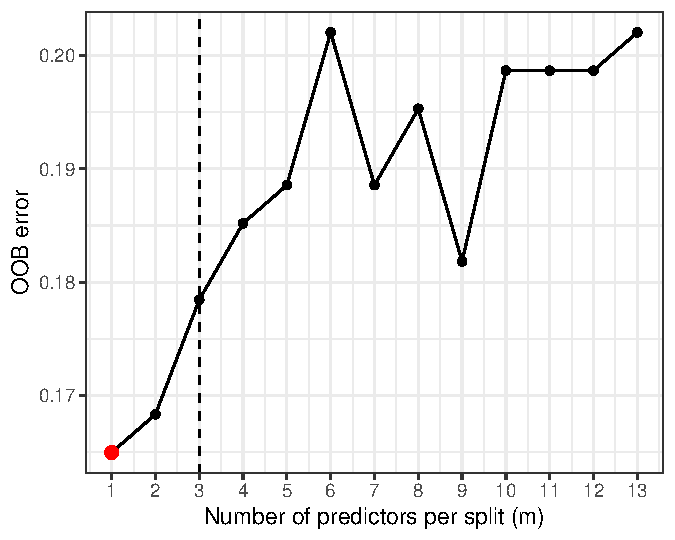
\includegraphics[width=\figscale\linewidth]{figures/heart_rf_mtry}}
        \end{column}
    \end{columns}
    Choose $m$ by the smallest OOB error, which needs no extra cross-validation.
\end{frame}


\begin{frame}{Parallel Versus Sequential Ensembles}
    \begin{itemize}
        \item \textbf{Bagging and random forests} grow trees in \textbf{parallel}, each on its own bootstrap sample, independently of the others
        \begin{itemize}
            \item Individual trees are deep: low bias, high variance
            \item Averaging reduces \textbf{variance}; bias stays about that of a single deep tree
        \end{itemize}
        \item \textbf{Boosting} grows trees \textbf{sequentially}, each fit to the residuals of the trees so far
        \begin{itemize}
            \item Individual trees are small: high bias, low variance
            \item Adding trees mainly reduces \textbf{bias}; the shrinkage $\lambda$ and the number of trees $B$ control the variance
        \end{itemize}
    \end{itemize}
\end{frame}


\begin{frame}{Boosting: Idea}
    \begin{itemize}
        \item Like bagging, boosting is a general approach that combines many trees
        \item Trees are grown \textbf{sequentially}: each tree is fit using information from the previously grown trees
        \item No bootstrap sampling: each tree is fit to a modified version of the original data, namely the current \textbf{residuals}
        \item \textbf{Learn slowly}: each new small tree is added with a shrinkage factor $\lambda$, slowly improving $\hat{f}$ in areas where it does not perform well
    \end{itemize}
\end{frame}


\begin{frame}{Boosting Algorithm for Regression Trees}
    \begin{enumerate}
        \item Set $\hat{f}(\mathbf{x}) = 0$ and $r^{(i)} = y^{(i)}$ for all $i$ in the training set
        \item For $b = 1, \dots, B$, repeat:
        \begin{enumerate}[(a)]
            \item Fit a tree $\hat{f}^{(b)}$ with $d$ splits ($d + 1$ leaves) to the training data $(\mathbf{X}, \mathbf{r})$
            \item Update $\hat{f}$ by adding a shrunken version of the new tree
            \[
                \hat{f}(\mathbf{x}) \leftarrow \hat{f}(\mathbf{x}) + \lambda\, \hat{f}^{(b)}(\mathbf{x})
            \]
            \item Update the residuals
            \[
                r^{(i)} \leftarrow r^{(i)} - \lambda\, \hat{f}^{(b)}\big(\mathbf{x}^{(i)}\big)
            \]
        \end{enumerate}
        \item Output the boosted model
        \[
            \hat{f}(\mathbf{x}) = \sum_{b=1}^{B} \lambda\, \hat{f}^{(b)}(\mathbf{x})
        \]
    \end{enumerate}
\end{frame}


\begin{frame}{Why Fit the Residuals?}
    \begin{itemize}
        \item For squared-error loss $L\big(y, f(\mathbf{x})\big) = \tfrac{1}{2} \big( y - f(\mathbf{x}) \big)^2$, the negative gradient with respect to $f(\mathbf{x}^{(i)})$ is the residual
    \end{itemize}
    \[
        - \frac{\partial L}{\partial f(\mathbf{x}^{(i)})} = y^{(i)} - f\big(\mathbf{x}^{(i)}\big) = r^{(i)}
    \]
    \begin{itemize}
        \item Fitting a tree to the residuals and adding $\lambda$ times it is a gradient descent step in function space, with step size $\lambda$
        \item Boosting is therefore a stagewise way of minimising the training loss
        \item For classification, the same idea is applied with a different loss, such as the binomial deviance (gradient boosting)
    \end{itemize}
\end{frame}


\begin{frame}{Boosting: Tuning Parameters}
    \begin{columns}[T]
        \begin{column}{0.5\textwidth}
            \begin{itemize}
                \item \textbf{Number of trees} $B$: unlike bagging and random forests, too large a $B$ can overfit; choose by cross-validation
                \item \textbf{Shrinkage} $\lambda$: typically $0.01$ or $0.001$; a small $\lambda$ needs a large $B$
                \item \textbf{Depth} $d$: controls interaction order; $d = 1$ (stumps) gives an additive model $\sum_j f_j(x_j)$
            \end{itemize}
        \end{column}
        \begin{column}{0.5\textwidth}
            % figure produced by heart.R
            \centerline{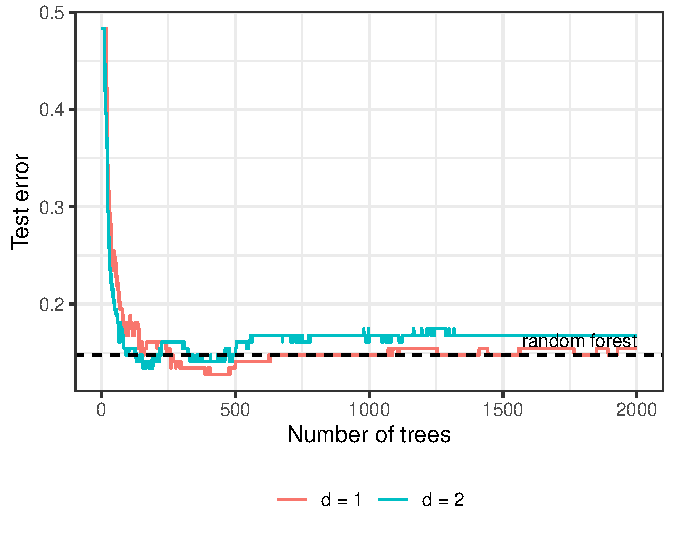
\includegraphics[width=\figscale\linewidth]{figures/heart_boost}}
        \end{column}
    \end{columns}
\end{frame}


% \begin{frame}{Bayesian Additive Regression Trees (BART): Idea}
%     \begin{itemize}
%         \item Combines ideas from both: $K$ trees as in bagging and random forests, each new tree fit to residuals as in boosting
%         \item Let $\hat{f}_k^{(b)}(\mathbf{x})$ be the prediction of tree $k$ at iteration $b$; the final model is $\hat{f}^{(b)}(\mathbf{x}) = \sum_{k=1}^{K} \hat{f}_k^{(b)}(\mathbf{x})$
%         \item Instead of fitting a new tree each time, iteration $b$ updates the $K$ trees one by one, and the $k$-th tree is a random \textbf{perturbation} of its previous version
%         \item Perturbations: change a leaf prediction, or grow or prune a branch; changes that improve the fit to the partial residual are favoured
%         \item Perturbations are modest, which avoids overfitting
%     \end{itemize}
% \end{frame}


% \begin{frame}{BART: Algorithm}
%     \begin{itemize}
%         \item When updating tree $k$ at iteration $b$, it is fit to the partial residual
%     \end{itemize}
%     \[
%         r^{(i)} = y^{(i)} - \sum_{k' < k} \hat{f}_{k'}^{(b)}\big(\mathbf{x}^{(i)}\big) - \sum_{k' > k} \hat{f}_{k'}^{(b-1)}\big(\mathbf{x}^{(i)}\big)
%     \]
%     \begin{itemize}
%         \item After a burn-in of $L$ iterations, the final prediction averages the remaining iterations
%     \end{itemize}
%     \[
%         \hat{f}(\mathbf{x}) = \frac{1}{B - L} \sum_{b=L+1}^{B} \hat{f}^{(b)}(\mathbf{x})
%     \]
%     \begin{itemize}
%         \item The procedure is a Markov chain Monte Carlo (MCMC) sampler from a Bayesian model; the burn-in iterations are discarded because early fits are poor
%     \end{itemize}
% \end{frame}


\begin{frame}{Summary of Tree Ensembles}
    \small
    \begin{center}
        \begin{tabular}{p{2cm}p{3.4cm}p{2.9cm}p{1.5cm}p{2cm}}
            \hline
            Method & Trees & Combination & Tuning & Reduces \\
            \hline
            Bagging & Deep trees on bootstrap samples & Average or majority vote & $B$ & Variance \\
            Random forest & As bagging, random $m$ of $p$ predictors per split & Average or majority vote & $B$, $m$ & Variance \\
            Boosting & Small trees grown sequentially on residuals & Sum of trees scaled by $\lambda$ & $B$, $\lambda$, $d$ & Bias \\
            % BART & $K$ small trees, randomly perturbed each iteration & Average over iterations after burn-in & $K$, $B$, $L$ & Variance and bias \\
            \hline
        \end{tabular}
    \end{center}
\end{frame}


\begin{frame}{Key Takeaways}
    \begin{itemize}
        \item Trees partition the predictor space into boxes and predict by the region mean or majority class; splits are chosen greedily by RSS, Gini or entropy
        \item Large trees overfit, so prune using cost complexity with $\alpha$ chosen by cross-validation
        \item Bagging reduces variance by averaging bootstrap trees, with OOB error as a free test error estimate
        \item Random forests decorrelate the trees by restricting the predictors considered at each split
%       \item Boosting grows small trees sequentially on residuals; BART adds a Bayesian perturbation scheme
        \item Boosting grows small trees sequentially on residuals
    \end{itemize}
\end{frame}
